% ---------------PLANTILLA INFORMES-------------- %

%---------Preambulo-------
\documentclass[11pt,letterpaper]{extarticle}        % Clase


\usepackage[utf8]{inputenc}                      % Codificación UTF-8
\usepackage[spanish]{babel}                      % Idioma del documento
\usepackage[left=2cm,right=2cm,bottom=3cm,top=2.5cm]{geometry}  % Dimesiones


% --------------------------LIBRERIAS-------------------------- %

\usepackage{enumitem}               % Enumeracion
\usepackage{fancyhdr}               % Encabezados y pies de pagina
\usepackage[ampersand]{easylist}    % Listas
\usepackage{amsmath}                % Fórmulas matemáticas
\usepackage{amssymb}                % Símbolos matemáticos
\usepackage{caption}                % Leyendas
\usepackage{color}                  % Colores
\usepackage{fancyhdr}               % Encabezados y pié de páginas
\usepackage{float}                  % Administrador de posiciones de objetos
\usepackage{geometry}               % Dimensiones y geometría del documento
\usepackage{graphicx}               % Propiedades extra para los gráficos
\usepackage[hidelinks]{hyperref}    % Permite añadir enlaces y referencias
\usepackage[makeroom]{cancel}       % Cancelar términos en fórmulas
\usepackage[version=4]{mhchem}      % Fórmulas químicas
\usepackage{multicol}               % Múltiples columnas
\usepackage{lipsum}                 % Permite crear textos dummy
\usepackage{longtable}              % Permite utilizar tablas en varias hojas
\usepackage{listings}               % Permite añadir código fuente
\usepackage{setspace}               % Cambia el espacio entre líneas
%\usepackage{subfig}
\usepackage{subfig}              % Permite agrupar imágenes
\usepackage{titlesec}               % Cambia el estilo de los títulos
\usepackage{url}                    % Permite añadir enlaces
\usepackage{wrapfig}                % Permite comprimir imágenes
\usepackage{pdfpages}

% LIBRERÍAS DEPENDIENTES
\usepackage{epstopdf}               % Convierte archivos .eps a pdf
\usepackage{multirow}               % Añade nuevas opciones a las tablas
\makeatletter

% INFORMACIÓN DEL DOCUMENTO
\newcommand{\nombredelinforme}{Reconocimiento y Pruebas en un
Ventilador Centrífugo}
\newcommand{\fecharealizacion}{\today}
\newcommand{\fechaentrega}{\today}
\newcommand{\nombreuniversidad}{Universidad de Chile}
\newcommand{\nombrefacultad}{Facultad de Ciencias Físicas y Matemáticas}
\newcommand{\departamentouniversidad}{Departamento de Ingeniería Mecánica}
\newcommand{\imagendeldepartamento}{images/departamentos/dimec}
\newcommand{\imagendeldepartamentoescala}{0.29}
\newcommand{\localizacionuniversidad}{Santiago, Chile}
\newcommand{\nombredelcurso}{Laboratorio de Máquinas}
\newcommand{\codigodelcurso}{ME5301}



% CONFIGURACIONES
\newcommand{\tiporeferencias}{apa}                  % Tipo de referencias
\newcommand{\nombreltformulas}{Lista de Fórmulas}   % Nombre de la lista de fórmulas
\newcommand{\nombrelttablas}{Lista de Tablas}       % Nombre de la lista de tablas
\newcommand{\nombreltfiguras}{Lista de Figuras}     % Nombre de la lista de figuras
\newcommand{\nombreltcontend}{Índice de Contenidos} % Nombre del índice de contenidos
\newcommand{\nombreltwtablas}{Tabla}                % Nombre de las tablas
\newcommand{\nombreltwfigura}{Figura}               % Nombre de las figuras
\numberwithin{equation}{section}                    % Ecuaciones con numero de seccion

% -------------------------FUNCIONES ESPECIALES------------------------- %
\newcommand{\grados}{^{\circ}}                      % Circulo superior para grados
\newcommand{\quotes}[1]{``#1''}                     % Citas
\newcommand{\quotesit}[1]{\textit{\quotes{#1}}}     % Citas italico

% ------ FORMATO ------------%

\fancypagestyle{Portada}{
\fancyhead[L] {\nombreuniversidad \\ \nombrefacultad \\ \nombredelcurso \: \codigodelcurso }
\fancyhead[R]{\includegraphics[scale=\imagendeldepartamentoescala]{\imagendeldepartamento}}
\cfoot{}
}

\fancypagestyle{NoPortadaNoEnumerada}{
\fancyhead[L] {\nombredelcurso \: \codigodelcurso \\ \nombredelinforme}
\fancyhead[R]{\nombreuniversidad \\ \departamentouniversidad}
\cfoot{}
}

\fancypagestyle{NoPortada}{
\fancyhead[L] {\nombredelcurso \: \codigodelcurso \\ \nombredelinforme}
\fancyhead[R]{\nombreuniversidad \\ \departamentouniversidad}
\cfoot{\thepage}
}






% --------------------------------DOCUMENTO-------------------------------- %
% INICIO DEL DOCUMENTO
\begin{document}

%BEGIN_FOLD
% PORTADA
\newpage
\pagestyle{fancy}
\thispagestyle{Portada}
\vspace*{5cm}
\begin{center}
	\vspace{1cm}
	\noindent\rule{\linewidth}{0.4pt}\\
	\Huge {\textbf{\nombredelinforme}}
		\vspace{0.3cm} 
	\noindent\rule{\linewidth}{0.3pt}
\end{center}
\vfill

% INTEGRANTES, PROFESORES Y FECHAS
\begin{minipage}{0.965\textwidth}
	\begin{flushright}
		\begin{tabular}{ll}
			Alumno: 
				& \begin{tabular}[t]{@{}l@{}}
					Daniel Mardini González\\
				\end{tabular} \\
			Curso:
				& \nombredelcurso \\
			Código:
				& \codigodelcurso \\
			Profesor: 
				& \begin{tabular}[t]{@{}l@{}}
					Ricardo Díaz S.\\
				\end{tabular} \\
			
			\multicolumn{2}{l}{Ayudante del laboratorio: Pedro Pino T.} \\
			& \\
			\multicolumn{2}{l}{Fecha de entrega: \fechaentrega} \\
			\multicolumn{2}{l}{\localizacionuniversidad}
		\end{tabular}
	\end{flushright}
\end{minipage}

% CONFIGURACIÓN DE PÁGINA Y ENCABEZADOS
\newpage
\renewcommand{\listfigurename}{\nombreltfiguras}    % Nombre del índice de figuras
\renewcommand{\listtablename}{\nombrelttablas}      % Nombre del índice de tablas
\renewcommand{\contentsname}{\nombreltcontend}      % Nombre del índice
\renewcommand{\tablename}{\nombreltwtablas}         % Nombre de la leyenda de las tablas
\renewcommand{\figurename}{\nombreltwfigura}        % Nombre de la leyenda de las figuras

\numberwithin{equation}{section}
\numberwithin{table}{section}
\numberwithin{figure}{section}


\pagestyle{fancy}
\thispagestyle{NoPortadaNoEnumerada}

% TABLA DE CONTENIDOS
\newpage
\tableofcontents        % Tabla de contenidos
\newpage
\listoffigures          % Índice de figuras
\listoftables           % Índice de tablas


\newpage
\setcounter{page}{1}
\pagestyle{NoPortada}

\section{Introducción}


\section{Objetivos}
\subsection*{Objetivo principal}
\subsection*{Objetivos secundarios}
\section{Antecedentes}
\section{Metodología}
\section{Memoria de cálculo}
\section{Resultados}

\begin{figure}[H]
\centering
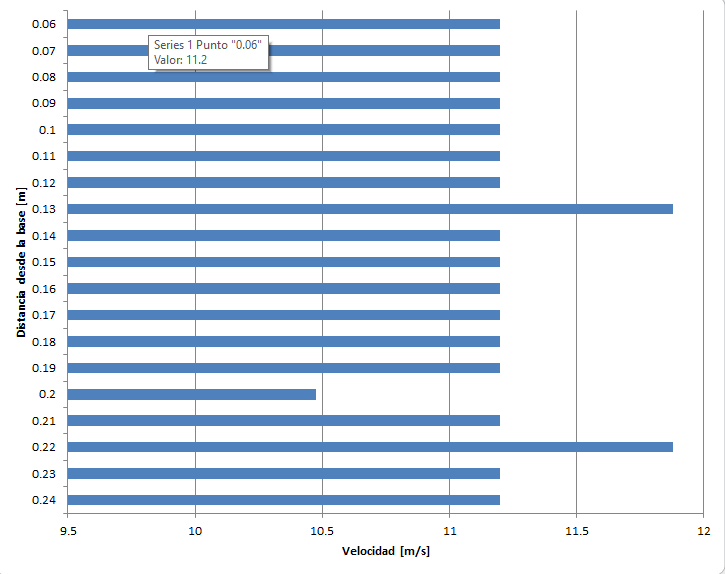
\includegraphics[width = 0.5\linewidth]{Perfil}
\caption{Perfil de velocidades del fluido}
\end{figure}

\begin{table}[H]
\centering
\caption{Calculo del coeficiente de centro.}
\label{t:C}
\resizebox{\textwidth}{!}{%
\begin{tabular}{|ccccccccc|}
\hline
$d_i$ {[}cm{]} & $d_i$ {[}m{]} & $r_i${[}m{]} & $P_{total}$ [mmCA] & $P_{estat}$ [mmCA] & $P_{din}$ {[}mCA{]} & $V${[}m/s{]} & $A_i$ {[}m$^2${]}  & $Q_i${[}m$^3$/s{]} \\ \hline
24                 & 0.24              & 0.09         & 39    & 31       & 0.008             & 11.2               & 0.002984513 & 0.033426546 \\
23                 & 0.23              & 0.08         & 42    & 34       & 0.008             & 11.2               & 0.002670354 & 0.029907962 \\
22                 & 0.22              & 0.07         & 44    & 35       & 0.009             & 11.879             & 0.002356194 & 0.027990163 \\
21                 & 0.21              & 0.06         & 45    & 37       & 0.008             & 11.2               & 0.002042035 & 0.022870795 \\
20                 & 0.2               & 0.05         & 46    & 39       & 0.007             & 10.477             & 0.001727876 & 0.018102336 \\
19                 & 0.19              & 0.04         & 51    & 43       & 0.008             & 11.2               & 0.001413717 & 0.015833627 \\
18                 & 0.18              & 0.03         & 56    & 48       & 0.008             & 11.2               & 0.001099557 & 0.012315043 \\
17                 & 0.17              & 0.02         & 57    & 49       & 0.008             & 11.2               & 0.000785398 & 0.008796459 \\
16                 & 0.16              & 0.01         & 58    & 50       & 0.008             & 11.2               & 0.000471239 & 0.005277876 \\
15                 & 0.15              & 0            & 58    & 50       & 0.008             & 11.2               & 0.00015708  & 0.001759292 \\
14                 & 0.14              & 0.01         & 57    & 49       & 0.008             & 11.2               & 0.000471239 & 0.005277876 \\
13                 & 0.13              & 0.02         & 57    & 48       & 0.009             & 11.879             & 0.000785398 & 0.009330054 \\
12                 & 0.12              & 0.03         & 57    & 49       & 0.008             & 11.2               & 0.001099557 & 0.012315043 \\
11                 & 0.11              & 0.04         & 59    & 51       & 0.008             & 11.2               & 0.001413717 & 0.015833627 \\
10                 & 0.1               & 0.05         & 59    & 51       & 0.008             & 11.2               & 0.001727876 & 0.019352211 \\
9                  & 0.09              & 0.06         & 56    & 48       & 0.008             & 11.2               & 0.002042035 & 0.022870795 \\
8                  & 0.08              & 0.07         & 52    & 44       & 0.008             & 11.2               & 0.002356194 & 0.026389378 \\
7                  & 0.07              & 0.08         & 48    & 40       & 0.008             & 11.2               & 0.002670354 & 0.029907962 \\
6                  & 0.06              & 0.09         & 46    & 38       & 0.008             & 11.2               & 0.002984513 & 0.033426546 \\ \hline
                   &                   &              &       &          &                   & Total              & 0.031258847 & 0.350983589 \\
                   &                   &              &       &          &                   & $V_{media}$                &      & 11.17215463 \\
                   &                   &              &       &          &                   &    $C$                &          & 0.997513806\\ \hline
\end{tabular}
}
\end{table}

\begin{table}[H]
\centering
\caption{Calculo de Potencia sobre el fluido y Potencia de freno}
\label{my-label}
\resizebox{\textwidth}{!}{%
\begin{tabular}{|cccccccccccc|}
\hline
\multicolumn{2}{|c}{$P_{pitot}${[}mmCA{]}} &  &  &  &  & \multicolumn{2}{c}{Presiones del ventilador{[}mmCA{]}} &  &  &  &  \\
$P_{Total}$ & $P_{est}$ & $P_{din}$ & $V${[}m/s{]} & $V_{media}$ & $Q${[}m/s{]} & Entrada & Salida & $H_t${[}mCA{]} & $N_f$ & $I${[}A{]} & $P_f$ \\
\hline
145 & 146 & 0.001 & 3.959797975 & 3.94995315 & 0.124091438 & 181 & 22 & -0.159 & -0.032884231 & 6.7 & 39.05956344 \\
137 & 142 & 0.005 & 8.854377448 & 8.832363751 & 0.277476891 & 173 & 36 & -0.137 & -0.063357223 & 6.9 & 89.94699839 \\
125 & 129 & 0.004 & 7.919595949 & 7.899906299 & 0.248182876 & 160 & 58 & -0.102 & -0.042191089 & 6.9 & 80.45104111 \\
114 & 120 & 0.006 & 9.699484522 & 9.675369725 & 0.303960704 & 146 & 82 & -0.064 & -0.032422475 & 6.9 & 98.532 \\
99 & 106 & 0.007 & 10.47664068 & 10.45059372 & 0.328315085 & 127 & 114 & -0.013 & -0.007113494 & 6.8 & 104.8843075 \\
87 & 94 & 0.007 & 10.47664068 & 10.45059372 & 0.328315085 & 113 & 140 & 0.027 & 0.014774179 & 6.7 & 103.3418912 \\
71 & 78 & 0.007 & 10.47664068 & 10.45059372 & 0.328315085 & 94 & 172 & 0.078 & 0.042680961 & 6.6 & 101.7994749 \\
58 & 65 & 0.007 & 10.47664068 & 10.45059372 & 0.328315085 & 76 & 204 & 0.128 & 0.070040551 & 6.4 & 98.71464232 \\
44 & 52 & 0.008 & 11.2 & 11.17215463 & 0.350983589 & 60 & 232 & 0.172 & 0.100615296 & 6.2 & 102.2325669 \\
38 & 46 & 0.008 & 11.2 & 11.17215463 & 0.350983589 & 50 & 248 & 0.198 & 0.115824584 & 6.1 & 100.5836545 \\
26 & 32 & 0.006 & 9.699484522 & 9.675369725 & 0.303960704 & 35 & 276 & 0.241 & 0.122090883 & 5.7 & 81.396 \\
14 & 21 & 0.007 & 10.47664068 & 10.45059372 & 0.328315085 & 21 & 312 & 0.291 & 0.159232816 & 5.2 & 80.20564688\\ \hline
\end{tabular}
}
\end{table}



\section{Análisis de resultados}
\section{Conclusiones}


		% REFERENCIAS
\newpage
\section{Anexo}

\begin{thebibliography}{x}
	\addcontentsline{toc}{section}{Referencias}
	
	\bibitem{b:Tabla} 
		S. Courtin V. (2006). \textit{APUNTES PARA EL CURSO ME53B: Laboratorio de Máquinas} Universidad de Chile.
	

\end{thebibliography}

\end{document}

